% !TEX TS-program = XeLaTeX
% use the following command: 
% all document files must be coded in UTF-8
\documentclass{textolivre}
% See more information on the repository: https://github.com/leolca/textolivre

% Metadata
\begin{filecontents*}[overwrite]{article.xmpdata}
    \Title{Matemática e Física em experiências de Robótica Livre: explorando o sensor ultrassônico}
    \Author{Marcelo Pires da Silva \sep Fernando da Costa Barbosa}
    \Language{pt-BR}
    \Keywords{Robótica Educacional Livre \sep Aprendizagem Criativa \sep Construcionismo \sep Ondas Ultrassônicas com robótica livre \sep Arduino no Ensino Básico}
    \Journaltitle{Texto Livre}
    \Journalnumber{1983-3652}
    \Volume{14}
    \Issue{3}
    \Firstpage{1}
    \Lastpage{19}
    \Doi{10.35699/1983-3652.2021.29629}

    \setRGBcolorprofile{sRGB_IEC61966-2-1_black_scaled.icc}
            {sRGB_IEC61966-2-1_black_scaled}
            {sRGB IEC61966 v2.1 with black scaling}
            {http://www.color.org}
\end{filecontents*}

\journalname{Texto Livre}
\thevolume{14}
\thenumber{3}
\theyear{2021}
\receiveddate{\DTMdisplaydate{2021}{2}{24}{-1}} % YYYY MM DD
\accepteddate{\DTMdisplaydate{2021}{5}{18}{-1}}
\publisheddate{\DTMdisplaydate{2021}{8}{24}{-1}}
% Corresponding author
\corrauthor{Marcelo Pires da Silva}
% DOI
\articledoi{10.35699/1983-3652.2021.29629}
%\articleid{NNNN} % if the article ID is not the last 5 numbers of its DOI, provide it using \articleid{} commmand
% list of available sesscions in the journal: articles, dossier, reports, essays, reviews, interviews, editorial
\articlesessionname{articles}
% Abbreviated author list for the running footer
\runningauthor{Silva e Barbosa}
\sectioneditorname{Daniervelin Pereira}
\layouteditorname{Anna Izabella M. Pereira}

\title{Matemática e Física em experiências de Robótica Livre: explorando o sensor ultrassônico}
\othertitle{Mathematics and Physics in Free Robotics experiments: exploring the ultrasonic sensor}
% if there is a third language title, add here:
%\othertitle{Artikelvorlage zur Einreichung beim Texto Livre Journal}

\author[1]{Marcelo Pires da Silva \orcid{0000-0002-5574-1055} \thanks{Email: \url{marte032@gmail.com}}}
\author[2]{Fernando da Costa Barbosa \orcid{0000-0001-8558-3521} \thanks{Email: \url{fcbarbosa@ufg.br}}}

\affil[1]{Rede Estadual de Educação do Estado de Goiás, Seduc-GO, Morrinhos, GO, Brasil.}
\affil[2]{Universidade Federal de Catalão, IMTec, Catalão, GO, Brasil.}

\addbibresource{article.bib}
% use biber instead of bibtex
% $ biber tl-article-template


% for spanish, use:
%\setdefaultlanguage{spanish}
%\gappto\captionsspanish{\renewcommand{\tablename}{Tabla}} % use 'Tabla' instead of 'Cuadro'
%\AfterEndPreamble{\crefname{table}{tabla}{tablas}\Crefname{table}{Tabla}{Tablas}}

% for languages that use special fonts, you must provide the typeface that will be used
% \setotherlanguage{arabic}
% \newfontfamily\arabicfont[Script=Arabic]{Amiri}
% \newfontfamily\arabicfontsf[Script=Arabic]{Amiri}
% \newfontfamily\arabicfonttt[Script=Arabic]{Amiri}
%
% in the article, to add arabic text use: \textlang{arabic}{ ... }

% for russian text we also need to define fonts with support for Cyrillic script
% \usepackage{fontspec}
% \setotherlanguage{russian}
% \newfontfamily\cyrillicfont{Times New Roman}
% \newfontfamily\cyrillicfontsf{Times New Roman}[Script=Cyrillic]
% \newfontfamily\cyrillicfonttt{Times New Roman}[Script=Cyrillic]
%
% in the text use \begin{russian} ... \end{russian}

% to use emoticons in your manuscript
% https://stackoverflow.com/questions/190145/how-to-insert-emoticons-in-latex/57076064
% using font Symbola, which has full support
% the font may be downloaded at:
% https://dn-works.com/ufas/
% add to preamble:
% \newfontfamily\Symbola{Symbola}
% in the text use:
% {\Symbola }

% reference itens in a descriptive list using their labels instead of numbers
% insert the code below in the preambule:
\makeatletter
\let\orgdescriptionlabel\descriptionlabel
\renewcommand*{\descriptionlabel}[1]{%
  \let\orglabel\label
  \let\label\@gobble
  \phantomsection
  \edef\@currentlabel{#1\unskip}%
  \let\label\orglabel
  \orgdescriptionlabel{#1}%
}
\makeatother
%
% in your document, use as illustraded here:
%\begin{description}
%  \item[first\label{itm1}] this is only an example;
%  % ...  add more items
%\end{description}
 

% custom epigraph - BEGIN 
%%% https://tex.stackexchange.com/questions/193178/specific-epigraph-style
\usepackage{epigraph}
\renewcommand\textflush{flushright}
\makeatletter
\newlength\epitextskip
\pretocmd{\@epitext}{\em}{}{}
\apptocmd{\@epitext}{\em}{}{}
\patchcmd{\epigraph}{\@epitext{#1}\\}{\@epitext{#1}\\[\epitextskip]}{}{}
\makeatother
\setlength\epigraphrule{0pt}
\setlength\epitextskip{0.5ex}
\setlength\epigraphwidth{.7\textwidth}
% custom epigraph - END


% if you use multirows in a table, include the multirow package
\usepackage{multirow}

% add line numbers for submission
%\usepackage{lineno}
%\linenumbers


\lstset{language=C++,keywordstyle={\bfseries\color{blue}}}

\begin{document}
\maketitle

\begin{polyabstract}
\begin{abstract}
Neste presente artigo, abordamos a aprendizagem de Matemática e Física por intermédio da Robótica Educacional em uma perspectiva livre, com a utilização de materiais livres, para que os estudantes criassem seus conhecimentos a partir da ideia do Construcionismo, alinhada à Espiral de Aprendizagem Criativa. A construção deste manuscrito foi possível a partir de uma pesquisa de campo, com um estudo de caso de caráter qualitativo, aplicada em uma turma de 9º ano de uma escola pública do estado de Goiás durante o segundo semestre de 2019, na qual foi utilizada a plataforma Arduino e peças de \textit{hardwares} livres. Por intermédio do desenvolvimento de robôs, com sequências de montagem, foi possível, imaginar, criar, brincar, compartilhar e refletir, perpassando a construção da Espiral de Aprendizagem Criativa. Dessa perspectiva, prepara-se o “terreno” para a aprendizagem de Matemática, Física, Engenharia, Tecnologias, Arte e Ciências, embutida ao processo de desenvolvimento do robô. Com as sequências desenvolvidas, aqui neste artigo, foi possível a aprendizagem de conceitos e habilidades, como: ondas ultrassônicas, velocidade média, conversão de unidades de medidas, funções e intervalos numéricos. Como resultado, pode-se salientar a importância do estudo da Matemática e das Ciências, alinhadas ao uso das tecnologias livres, encurtando a distância entre conhecimento curricular e o desenvolvimento tecnológico sustentável.

\keywords{Robótica Educacional Livre \sep Aprendizagem criativa \sep Construcionismo \sep Ondas ultrassônicas com Robótica Livre \sep Arduino no ensino básico}
\end{abstract}

\begin{english}
\begin{abstract}
In this article, we approach Mathematics and Physics learning through Educational Robotics in a free perspective, with the use of free materials, so that students could build up their knowledge from the idea of Constructionism, aligned with the Creative Learning Spiral. The construction of this manuscript was possible with/through a field research, with a qualitative case study, applied in a 9th grade class of a public school in the state of Goiás, Brazil, during the second semester of 2019, in which the Arduino platform and free hardware parts are used. Through the development of robots, with assembly sequences, it was possible to imagine, create, play, share and reflect, permeating the construction of the Creative Learning Spiral. From this perspective, the “ground” is prepared for the learning of Mathematics, Physics, Engineering, Technologies, Art and Sciences, embedded in the robot development process. With the sequences developed here in this article, it was possible for students to learn concepts and skills, such as: ultrasonic waves, average speed, conversion of measurement units, functions and numerical intervals. As a result, it is possible to emphasize the importance of studying Mathematics and Science, aligned with the use of free technologies, shortening the distance between curricular knowledge and sustainable technological development.

\keywords{Free Educational Robotics \sep Creative learning \sep Constructionism \sep Ultrasonic waves with free robotics \sep Arduino in Basic Education}
\end{abstract}
\end{english}

% if there is another abstract, insert it here using the same scheme
\end{polyabstract}


\section{Introdução}\label{sec-intro}
Neste trabalho\footnote{Este artigo é resultado de uma dissertação de mestrado do PROFMAT da UFG. A coleta de dados seguiu normas éticas, sendo um dos objetivos específicos do projeto intitulado “Investigações relativas ao processo de ensino-aprendizagem de Matemática”, cadastrado na plataforma Brasil com número 91278218.7.0000.8409, em que os autores são pesquisadores assistentes.}, abordarmos alguns relatos sobre a utilização da Robótica Educacional Livre, que foram obtidos por meio de um estudo de caso a partir de uma pesquisa qualitativa, desenvolvida em uma escola da rede pública do estado de Goiás durante o ano letivo de 2019, com a participação de quatro estudantes da instituição, sendo uma menina e três meninos. Dois participantes tinham 14 anos e os outros dois, 15 anos de idade.

A utilização da Robótica Educacional Livre, como desenvolvido em nossa pesquisa, foi uma alternativa para a implementação de uma nova forma de trabalhar o currículo tradicional,  visando à criação de mecanismos e situações que permitiam os participantes envolvidos a criar, explorar, desenvolver, recriar novas ferramentas e, consequentemente, gerar ideias inovadoras e criativas, por meio de uma Filosofia que permitisse o compartilhamento de ideias e projetos, uma filosofia de perspectiva Livre, como a filosofia do projeto GNU\footnote{Projeto GNU - O projeto GNU foi concebido em 1983 como uma maneira de trazer de volta o espírito cooperativo que
prevalecia na comunidade de computação nos seus primórdios — para tornar a cooperação possível novamente ao remover
os obstáculos à cooperação impostos pelos donos de software proprietário \cite{foundation}.}.

No desenvolver de nossa pesquisa, elaboramos aulas e sequências didáticas, em que os participantes desta pesquisa realizavam a montagem e a programação dos robôs. Entrelaçado ao desenvolvimento dessas aulas, identificamos o envolvimento dos participantes que socializavam, trocavam ideias, orientavam uns aos outros para o desenvolver das aulas e projetos, criavam novas ideias e compartilhavam o que aprendiam, refletiam.

Por meio dessas observações, identificamos com o que \textcite{resnick2020} chama de espiral da aprendizagem criativa. Segundo o autor,

\begin{quote}
A espiral de aprendizagem criativa é o motor do pensamento criativo. À medida que as crianças do jardim de infância percorrem a espiral, elas desenvolvem e refinam suas habilidades como pensadoras criativas, aprendem a desenvolver as próprias ideias, testá-las, experimentar alternativas, obter as opiniões de outras pessoas e criar ideias baseadas em suas experiências \cite[p. 39]{resnick2020}.
\end{quote}

Nesse sentido, estendemos esse entendimento aos participantes do projeto de pesquisa, que possuíam entre 14 e 15 anos. Ao mesmo tempo em que os participantes de nossa pesquisa viam novas possibilidades de criação de modelo robóticos e suas aplicações, necessariamente, eles estavam percorrendo a espiral de aprendizagem criativa, como observamos na \Cref{fig1}.

\begin{figure}[htbp]
 \centering
 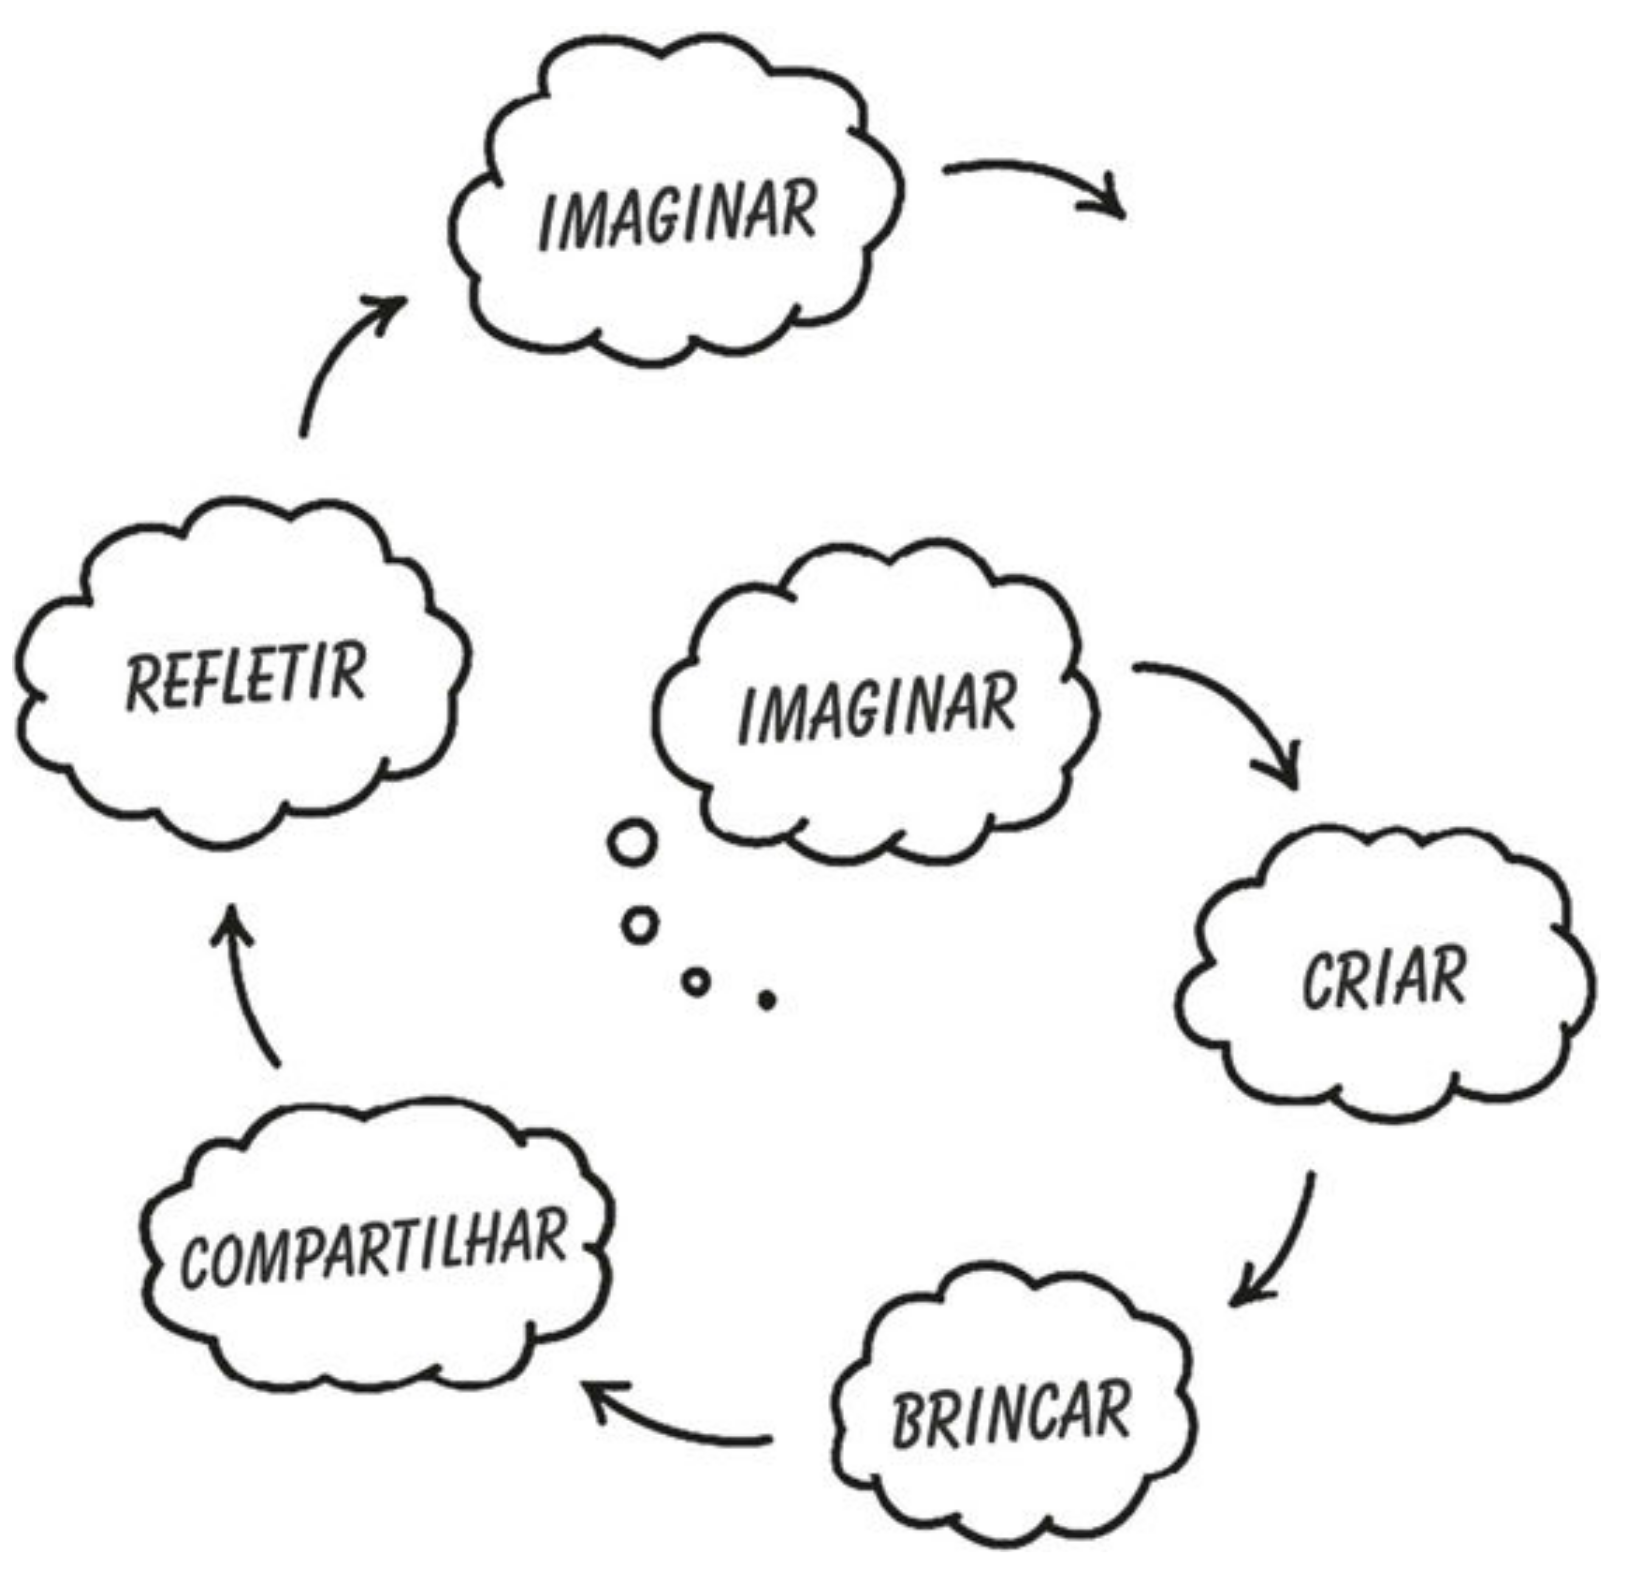
\includegraphics[width=0.5\textwidth]{fig-001.png}
 \caption{Espiral de Aprendizagem Criativa}
 \label{fig1}
 \source{\textcite[p. 40]{resnick2020}.}
\end{figure}

Em primeiro momento, durante as primeiras aulas de robóticas, especificamente, durante a montagem do robô seguidor de linha, não foi identificada a utilização da espiral de aprendizagem criativa no projeto pelos participantes. Mas, a partir das aulas de montagem dos Robôs com sensor ultrassônico das quais aqui trataremos, observamos que os participantes realizavam ações que perpassavam a Espiral de Aprendizagem Criativa. Portanto, para que ocorresse o acesso, por parte dos estudantes, à Espiral Criativa de Aprendizagem, foi necessário um contato dos participantes com os materiais robóticos utilizados na pesquisa, bem como a realização de algumas aulas de montagem do robô seguidor de linha transistorizado e alguns circuitos simples com Arduino, como ligar um LED por determinado período de tempo.

A partir dessa linha de pensamento, utilizamos a plataforma Arduino em conjunto com a Robótica Educacional Livre para desenvolver uma pesquisa sobre como a Robótica Educacional Livre desenvolvida em conjunto com a plataforma Arduino poderia desenvolver e agregar na aprendizagem de Matemática e Física.

Nesse sentido, a pesquisa foi desenvolvida com o caráter qualitativo, utilizando-se do método de Estudo de Caso, com análise qualitativa dos dados. Nosso estudo baseou-se em um estudo de caso único, com subunidades integradas de análise, tendo como caso principal as aulas desenvolvidas de Robótica Pedagógica Livre, que se dividiu em duas subunidades de análise: as aulas de desenvolvimento e montagem do Robô seguidor de linha, bem como as aulas tratadas aqui neste artigo, com a construção e desenvolvimento de robôs ultrassônicos, por meio de Arduino e sensor ultrassônico. Para a obtenção e armazenamento de dados, utilizaram-se Documentação em forma de questionários, registro em arquivos em forma de imagens/fotografias, vídeos, arquivos de áudios, entrevistas, observações diretas, observação participante e os artefatos físicos produzidos pelos participantes. Utilizamos como estratégia geral para análise de dados a proposição teórica de tratar os dados “a partir do zero”. Para o modelo de análise específicas, utilizamos modelos lógicos, de nível individual para nível organizacional.

Para \textcite[p. 139]{yin2015}, “brincar” com os dados nos permite obter alguns \textit{insights} e padrões. Para o autor,

\begin{quote}
Algumas dessas criações preliminares – como matrizes, representações, tabulações, notas ou diagramas – irão ajudá-lo a seguir em direção a uma estratégia analítica geral. A estratégia necessária deve seguir um ciclo (ou ciclos repetidos)envolvendo suas questões de pesquisa originais, os dados, seu manuseio e sua interpretação justificáveis dos dados e sua capacidade de expor algumas descobertas e tirar algumas conclusões \cite[p. 140]{yin2015}.
\end{quote}

Quando tratamos os dados “a partir do zero”, para \textcite{yin2015}, realizando

\begin{quote}
a sua ‘brincadeira com os dados’ ou percebendo um padrão pela primeira vez, agora você pode descobrir que alguma parte dos seus dados sugere um ou dois conceitos úteis. Esse \textit{insight} pode ser o início de um caminho analítico, levando-o mais adiante e possivelmente sugerindo relações adicionais \cite[p. 141]{yin2015}.
\end{quote}

Este artigo está organizado em cinco tópicos em que trataremos, na \cref{sec-roboticaeducacional}, sobre um breve histórico da Robótica Educacional, com o Construcionismo de Papert, sobre as definições de Robótica Livre e Robótica Educacional Livre. Na \cref{sec-desenvolvimento}, abordaremos sobre como desenvolvemos e percorremos a Espiral de Aprendizagem, por meio do trabalho com a Robótica Educacional Livre. Na \cref{sec-4}, faremos uma breve reflexão sobre os sentimentos e aprendizagens dos participantes durante o desenvolvimento da Robótica Educacional Livre e, na \cref{sec-5}, finalizaremos com algumas considerações finais e ideias de projetos futuros.

\section{Robótica Educacional}\label{sec-roboticaeducacional}
A Robótica Educacional (RE), como a conhecemos, foi idealizada e desenvolvida pelo matemático sul-africano Seymour Papert, na década de 1960. Papert via o computador com um objeto que poderia ser utilizado para a construção do conhecimento. Segundo ele, 

\begin{quote}
eu já indiquei uma razão para acreditar que a presença do computador deve ter efeitos mais fundamentais no desenvolvimento intelectual do que aqueles efeitos produzidos por outras tecnologias, inclusive a televisão e até mesmo a imprensa. A metáfora do computador como uma entidade que ’fala’ uma linguagem matemática coloca o aprendiz numa nova qualidade de relacionamento com um importante domínio do conhecimento. Mesmo o melhor em matéria de televisão educativa está limitado a oferecer progressos somente quantitativos para os tipos de aprendizagem que existiam sem a televisão. ‘Vila Sésamo’ pode oferecer explicações melhores ou mais envolventes que as que a criança recebe dos pais ou de professores de pré-primário, mas a criança continua na posição de ouvinte das explicações \cite[p. 36]{papert1980}.
\end{quote}

Para Papert, o computador é uma ferramenta de construção de conhecimento, que romperá a barreira da educação, como diria Paulo Freire, do tipo bancária. Na percepção de Papert, 

\begin{quote}
A educação tradicional codifica o que pensa que os cidadãos precisam saber e parte para alimentar as crianças com esse ‘peixe’. O construcionismo é construído sobre a suposição de que as crianças farão melhor descobrindo (‘pescando’) por si mesmas o conhecimento específico de que precisam: a educação organizada ou informal poderá ajudar mais se certificar-se de que elas estarão sendo apoiadas moral, psicológica, material e intelectualmente em seus esforços \cite[p. 135]{papert1980}.
\end{quote}

Seymour Papert, no início dos anos 60, trabalhou com Jean Piaget na Universidade de Genebra. Analisando entrevistas feitas com milhares de crianças, Piaget descobriu como as crianças construíam ativamente seu conhecimento a partir das interações feitas com objetos e pessoas, construindo seu conhecimento e não o recebendo passivamente.

A partir da aprendizagem com Jean Piaget, Papert propôs uma forma diferente de como as crianças desenvolvem suas ideias. Além de defender que as crianças não recebem as ideias de forma passiva, defendeu que elas constroem suas ideias e conhecimentos, de forma mais eficaz, por meio de interações que elas fazem com o mundo, através, por exemplo, de materiais concretos. A essa abordagem Papert deu o nome de Construcionismo.

\begin{quote}
Ele chamou sua abordagem de construcionismo, porque une dois tipos de construção: à medida que as crianças constroem coisas no mundo, elas constroem novas ideias em suas mentes, o que as incentiva a construir novas coisas no mundo e assim por diante, em uma espiral infinita de aprendizagem \cite[p. 68]{resnick2020}.
\end{quote}

A partir da teoria do Construcionismo, em conjunto com a robótica, o estudante poderá fazer novas descobertas por si, criando, refletindo, elaborando e aperfeiçoando aquele conhecimento que internalizou, ou mesmo buscando novos conhecimentos para aprimorar o seu aprendizado. Esse processo nos leva, como mostrado anteriormente, à Espiral de Aprendizagem Criativa, que, segundo \textcite{resnick2020}, 

\begin{quote}
é entendida como o motor criativo das crianças, onde elas desenvolvem e refinam suas habilidades como pensadoras criativas, aprendem e desenvolvem ideias, testam, experimentam alternativas, obtém opiniões de outras pessoas e criam ideias com suas experiências \cite[p. 41]{resnick2020}.
\end{quote}

\subsection{Robótica Educacional Livre}
Na Robótica Educacional, temos uma vertente chamada de Robótica Educacional Livre ou Robótica Pedagógica Livre, que é um tipo de robótica que pressupõe a utilização de materiais e \emph{softwares} livres. O desenvolver da Robótica Livre se utiliza de materiais livres, tanto \emph{software} quanto \emph{hardware}, que são materiais que possuem licenciamentos baseados nas definições de \emph{software} livre. Segundo \textcite{association}, \emph{hardwares} livres são,

\begin{quote}
[…] artefatos tangíveis — máquinas, dispositivos ou outros objetos físicos — cujo projeto foi disponibilizado ao público de modo que qualquer um pode construir, modificar, distribuir e utilizar estes artefatos. É intenção desta definição auxiliar no desenvolvimento de guias gerais para o desenvolvimento e validação de licenças para Open Source Hardware \cite{association}.
\end{quote}

Os \emph{softwares} livres trazem algumas liberdades para com o usuário. \textcite{stallman2002} define essas liberdades:

\begin{quote}
Primeira Liberdade é a liberdade de executar o programa como você desejar, para qualquer propósito. \newline
Liberdade 1 é a liberdade de estudar como o programa funciona, e adaptá-lo às suas necessidades. \newline 
Liberdade 2 é a liberdade de redistribuir cópias de modo que você possa ajudar outros. \newline 
E liberdade três é a liberdade para ajudar a construir a sua comunidade, publicando uma versão melhorada para que outros possam obter o benefício do seu trabalho \cite[p. 165, tradução dos autores]{stallman2002}\footnote{\emph{a program is “free software” for you, a particular user, if you have the following freedoms: \newline
First, Freedom Zero is the freedom to run the program for any purpose, any way you like. \newline
Freedom One is the freedom to help yourself by changing the program to suit your needs. \newline
Freedom Two is the freedom to help your neighbor by distributing copies of the program. \newline
And Freedom Three is the freedom to help build your community by publishing an improved version so others can get the
benefit of your work} \cite[p. 165]{stallman2002}.}.
\end{quote}

Dentro da perspectiva de visão de robótica praticada com os ideais da filosofia GNU\footnote{GNU – GNU is Not a Unix – Trocadilho feito por desenvolvedores para se referir ao projeto GNU.} (ideais do \emph{Software} Livre), criou-se a Robótica Educacional Livre. Uns dos primeiros a utilizar os ideais e da filosofia Gnu nessa proposta de robótica é o pesquisador Danilo César. Para \textcite{cesar2013}, a Robótica Pedagógica Livre é

\begin{quote}
[...] o conjunto de processos e procedimentos envolvidos em propostas de ensino e de aprendizagem que utilizam os kits pedagógicos e os artefatos cognitivos baseados em soluções livres e em sucatas como tecnologia de mediação para a construção do conhecimento \cite{cesar2013}.
\end{quote}

Em nossa pesquisa, utilizamos a plataforma Arduino e materiais elétricos/eletrônicos livres, bem como sucatas eletrônicas. Para o desenvolvimento do \emph{software} controlador do robô, utilizamos  um computador com MS Windows e outro com Debian GNU/Linux, além da IDE\footnote{IDE – Integrated Development Environment – Ambiente de Desenvolvimento Integrado} Arduino.

\subsection{Robótica Educacional Livre desenvolvida com Arduino}
O Arduino é uma plataforma de prototipagem de licenciamento jurídico livre, possuindo apenas restrição de registro a marca Arduino, que surgiu na Itália, em 2005. É uma placa que possui um microcontrolador\footnote{Microcontrolador: o microcontrolador consiste em um único circuito integrado que reúne um núcleo de processador, memórias voláteis e não voláteis e diversos periféricos de entrada e de saída de dados.} que é capaz de “ler” e “escrever” valores analógicos e digitais, sendo controlada por um \textit{software}, que o usuário cria em sua própria IDE de desenvolvimento (\Cref{fig2}).

\begin{figure}[htbp]
 \centering
 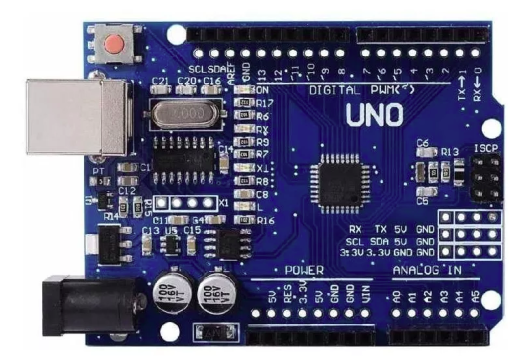
\includegraphics[width=0.5\textwidth]{fig-002.png}
 \caption{Arduino Uno}
 \label{fig2}
 \source{Arquivo pessoal.}
\end{figure}

A placa possui portas de pinagem enumeradas e identificadas, sendo A0, A1, portas analógicas, 1, 2, 3…, portas digitais, e portas que possuem o símbolo $\sim$, que são portas que podem ser utilizadas como PWM\footnote{PWM - Pulse Width Modulation" ou Modulação de Largura de Pulso, através da largura do pulso de uma onda quadrada é possível o controle de potência ou velocidade.}. A alimentação da placa pode ser feita via USB ou por bateria de 9 V 9F22.

\begin{figure}[htbp]
 \centering
 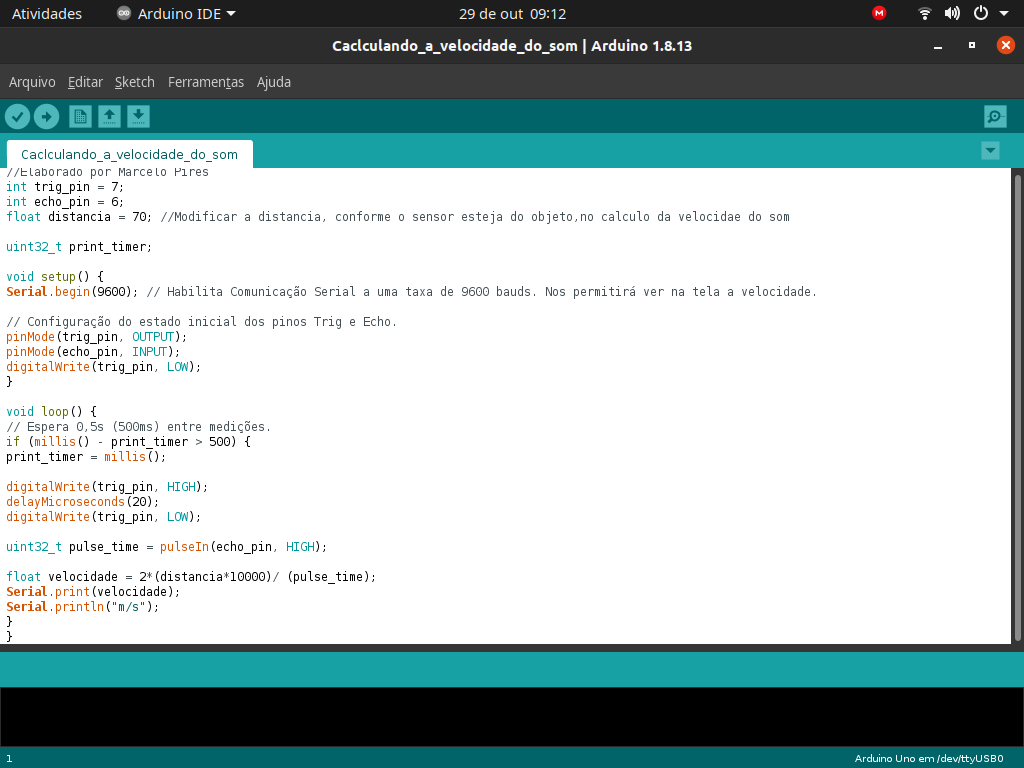
\includegraphics[width=\textwidth]{fig-003.png}
 \caption{IDE Arduino.}
 \label{fig3}
 \source{Arquivo pessoal.}
\end{figure}

O \emph{software} do robô pode ser escrito na IDE (\Cref{fig3}), por meio da linguagem de programação C e algumas funções de definições que a própria plataforma possui, como as funções, \emph{analogRead}, \emph{digitalRead}, \emph{analogWrite}, \emph{digitalWrite}, \emph{pinMode}, entre outras.

Para a construção de robôs ou autômatos, são utilizados sensores, atuadores e peças eletrônicas, que são montados em uma placa de testes e prototipagem, chamada de \emph{Protoboard} ou \emph{Breadboard}, como podemos observar na \Cref{fig4}.

\begin{figure}[htbp]
 \centering
 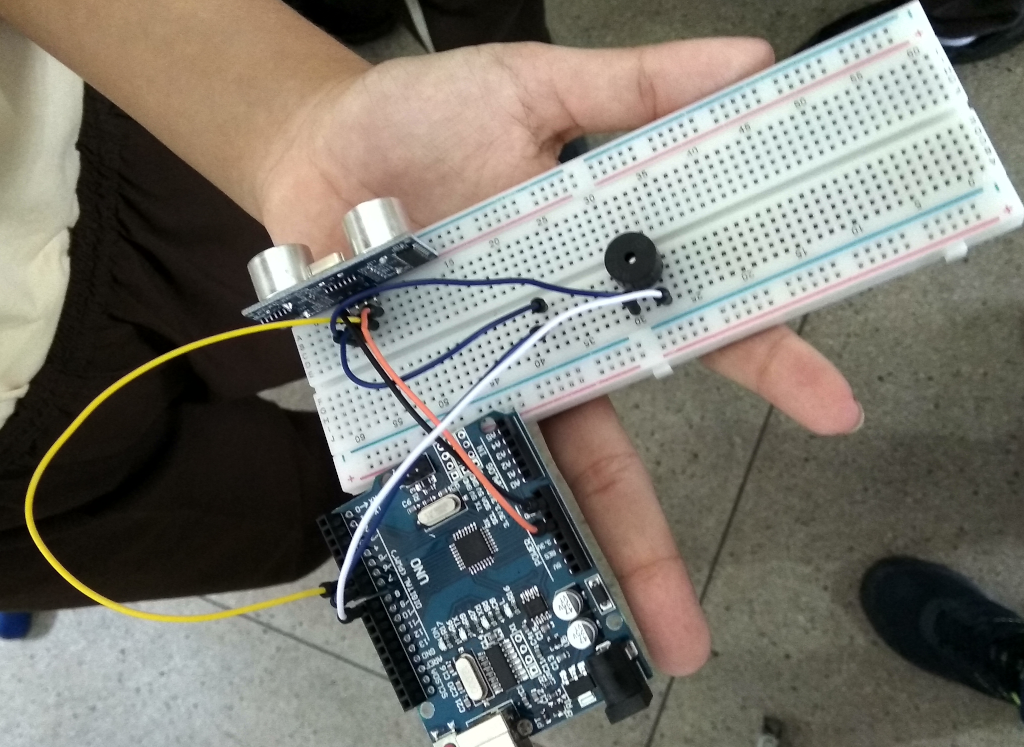
\includegraphics[width=0.5\textwidth]{fig-004.png}
 \caption{Prototipagem em uma \emph{Protoboard}.}
 \label{fig4}
 \source{Arquivo pessoal.}
\end{figure}

A \emph{Protoboard} em conjunto com a plataforma Arduino permite ao participante fazer, criar, recriar, testar e inovar, que é o material que precisávamos para o desenvolvimento da aprendizagem criativa, defendida por \textcite{resnick2020}.

A Robótica Educacional Livre desenvolvida com Arduino, em comparação a outros \textit{kits} robóticos, a priori, pode ser um pouco complexa em sua montagem e desenvolvimento de \emph{software}. Quanto ao desenvolvimento de \textit{software}, existe um programa, \emph{Scratch For} Arduino, que utiliza o \emph{Scratch}\footnote{Scratch: Linguagem de programação baseada em blocos, desenvolvida por Mitchel Resnick, no Mit MediaLab.} para a programação do \emph{software}.

Em nossa pesquisa, utilizamos a própria IDE do Arduino, pois haveria uma gama maior de conteúdo dentro do currículo matemático para trabalho, além de ser um material robótico caracterizado como \emph{software} livre.

\section{Desenvolvimento de um robô com sensor ultrassônico}\label{sec-desenvolvimento}
Os objetos robóticos aqui apresentados foram desenvolvidos por quatro participantes de um projeto de pesquisa qualitativo, divididos em duplas, durante o segundo semestre do ano de 2019, em uma instituição pública de ensino. Os projetos de robótica livre utilizaram sucatas e objetos de \emph{hardwares} livres, com o grupo de estudantes citados. O grupo de pesquisa era composto por um pesquisador e quatro participantes de uma turma de 9º ano da referida instituição pública. Foi feita a montagem de um robô seguidor de linha transistorizado, robô seguidor de linha controlado por Arduino e robôs utilizando o sensor ultrassônico, como abordaremos por aqui nesta seção.

A escolha da montagem do robô seguidor de linha foi por se tratar um robô básico, pelo qual os participantes têm primeiro contato com a robótica e os materiais de desenvolvimento. Normalmente, faz-se  um projeto-piloto quando se começa a estudar Arduino e, nesse caso especial, deu-se como parte de uma pesquisa de mestrado desenvolvida na instituição pública de ensino básico. Portanto, o desenvolvimento do robô ultrassônico deu-se após a confecção de robôs seguidores de linha pelos estudantes. Para o robô ultrassônico, utilizamos um sensor HC-SR04, uma placa Arduino UNO e \emph{Jumpers} (macho-fêmea). A criação do robô se deu em duas partes: construção do \emph{hardware} do robô (parte concreta do robô) e construção do \emph{software} de controle do robô (parte abstrata).

Por meio da construção do \emph{hardware} do robô, o participante observa e compreende as partes de alimentação e controle de cada item do robô, fazendo com que ele tenha atenção durante a montagem. A montagem permite ao participante conhecer o princípio de funcionamento do robô. 

No caso do desenvolvimento do robô com sensor ultrassônico, a primeira parte de sua montagem possui apenas quatro fios, um sensor e a placa de controle Arduino.

\begin{figure}[htbp]
 \centering
 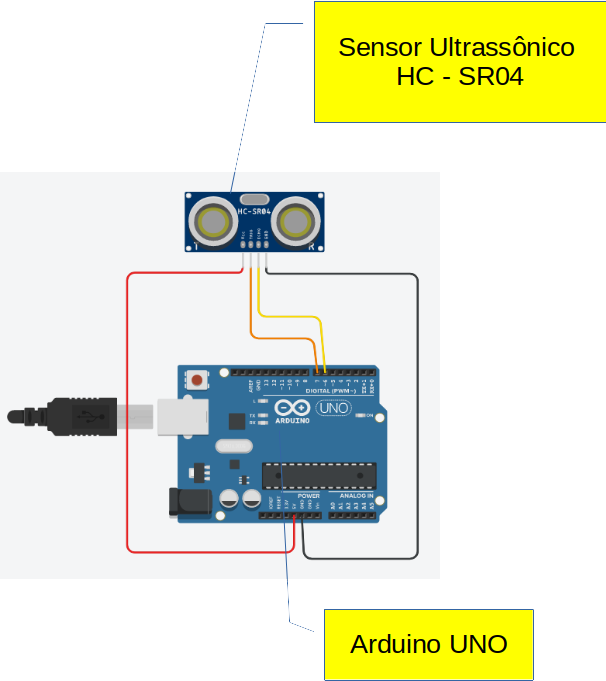
\includegraphics[width=0.5\textwidth]{fig-005.png}
 \caption{Robô com sensor ultrassônico e Arduino.}
 \label{fig5}
 \source{Arquivo pessoal.}
\end{figure}

A \Cref{fig5} mostra o \textit{hardware} do robô com sensor ultrassônico. Observa-se que sua construção contém apenas 4 fios, sendo dois deles para alimentação (VCC – 5 V – Vermelho e GND – 0 V – Preto) e outros dois fios com as seguintes características: um utilizado para enviar o sinal ao \emph{trigger}, para que o sensor envie as ondas ultrassônicas de 40 Khz, e o outro fio, echo, envia, caso necessário, o sinal de retorno percebido pelo sensor ao Arduino. O restante do processo é feito através de \emph{software} programado e compilado pela IDE e gravado no Arduino. A alimentação do robô poderá ser feita através do cabo USB ou bateria 9 V modelo 6F22.

\subsection{Desenvolvendo o robô para cálculo da velocidade do som}\label{sec-3.1}
Na robótica, temos condições de explorar mais que os componentes e seu funcionamento, como também conceitos científicos da Matemática e da Física. Nesse caso, o projeto permitiu o desenvolvimento do robô para cálculo da velocidade de som, utilizando-se o \textit{hardware} mostrado na \Cref{fig5}. Com esse \emph{hardware}, tínhamos uma ferramenta que era capaz de enviar/produzir Ondas Ultrassônicas em frequência de 40 KHz e também perceber a existência de retorno da onda ultrassônica, quando era refletida por algum objeto a sua frente. O \emph{software} para o controle do robô para o cálculo da velocidade é mostrado na \Cref{lst01} a seguir.

\begin{lstlisting}[label=lst01, caption={Programa para o cálculo da velocidade do som no Arduino.}, source={Arquivo pessoal.}]
//Elaborado por Marcelo Pires
int trig_pin = 7;
int echo_pin = 6;
float distancia = 70; //Modificar a distancia em centímetros (cm), conforme o sensor esteja do objeto,no cálculo da velocidade do som
 
uint32_t print_timer;
 
void setup() {
Serial.begin(9600); // Habilita Comunicação Serial a uma taxa de 9600 bauds. Nos permitirá ver na tela a velocidade.
 
// Configuração do estado inicial dos pinos Trig e Echo.
pinMode(trig_pin, OUTPUT);
pinMode(echo_pin, INPUT);
digitalWrite(trig_pin, LOW);
}
 
void loop() {
// Espera 0,5s (500ms) entre medições.
if (millis() - print_timer > 500) {
print_timer = millis();
 
digitalWrite(trig_pin, HIGH);
delayMicroseconds(20);
digitalWrite(trig_pin, LOW);
 
uint32_t pulse_time = pulseIn(echo_pin, HIGH);

float velocidade = 2*(distancia*10000)/ (pulse_time);
Serial.print(velocidade);
Serial.println("m/s");
}
}
\end{lstlisting} %stopzone

Para o cálculo da velocidade de som, baseamo-nos na ideia de velocidade média, ou a velocidade média de determinado corpo/partícula/onda, que é dada pela razão do espaço percorrido pelo tempo gasto nesse percurso, como mostra a \Cref{eq01}. 

\begin{equation}\label{eq01}
V_m = \frac{d}{t}
\end{equation}

Definimos a distância que algum objeto deveria ficar à frente do sensor ultrassônico do robô e declaramos essa distância, em centímetros, no \emph{software}, como \emph{float distancia} = 70. Restam-nos ainda duas variáveis: tempo e velocidade. Como queríamos encontrar a velocidade, logo utilizamos o \emph{software} mostrado na \Cref{lst02} para o cálculo do tempo:

\begin{lstlisting}[label=lst02, caption={Calculando o tempo de percurso da Onda Ultrassônica.}, source={Arquivo pessoal.}]
if (millis() - print_timer > 500) {
print_timer = millis();
 
digitalWrite(trig_pin, HIGH);
delayMicroseconds(20);
digitalWrite(trig_pin, LOW);
 
uint32_t pulse_time = pulseIn(echo_pin, HIGH);
\end{lstlisting} %stopzone


O tempo de percurso da onda ultrassônica, do sensor ao objeto e do objeto ao sensor, é o tempo obtido pela variável \lstinline{pulse_time}. Atente-se ao fato que esse tempo está dobrado, já que, para o cálculo da velocidade do som, é necessário somente o tempo de percurso da Onda, do sensor ao Objeto posto à frente. Para calcular somente o tempo de percurso da Onda Ultrassônica do sensor ao Objeto, e já calculando a velocidade do som, em m/s, utilizamos o código mostrado na \Cref{lst03}.

\begin{lstlisting}[label=lst03, caption={Calculando a Velocidade do Som no Ambiente em que se encontra o Robô.}, source={Arquivo pessoal.}]
float velocidade = 2*(distancia*10000)/ (pulse_time);
Serial.print(velocidade);
Serial.println("m/s");
\end{lstlisting} %stopzone

O multiplicar por dois no código nos retorna ao tempo de percurso entre o sensor e o Objeto. Já o multiplicar por 10000 (\lstinline{*10000}) faz a conversão da distância que estava em cm (centímetro = $10^{-2}$m) para m (metro) e, ao mesmo tempo, do tempo que é obtido em μs (microssegundos = $10^{-6}$s) para segundos, retornando a velocidade na tela por meio de \lstinline{Serial.print(velocidade);} e \lstinline{Serial.println("m/s");}, em m/s., terminando o processo de cálculo da velocidade do som pelo robô.

\subsection{Imaginar, criar, brincar, compartilhar e refletir: transformando o robô de cálculo da velocidade do som em robô medidor de distância por ondas ultrassônicas}\label{sec-3.2}
Imaginando e refletindo, por meio do desenvolvimento do robô para cálculo da velocidade do som, criou-se um novo robô, utilizando-se da velocidade média obtida na etapa anterior, que permitia o cálculo da distância de objetos ao sensor, por meio do uso das ondas ultrassônicas. 

Essa ideia surgiu quando os participantes estavam testando o robô construído na \cref{sec-3.1}. Segundo eles, se é possível obter a velocidade do som, fixando a distância e obtendo o tempo de percurso da Onda Ultrassônica, logo também seria possível obter a distância, sem modificar o \textit{hardware} do robô, fixando a velocidade do som e obtendo, da mesma maneira, o tempo de percurso da Onda Ultrassônica. Como definimos a velocidade média como sendo a razão entre a distância pelo tempo, logo isolando a variável que representa a distância na fórmula, podemos adequá-la no \textit{software} do Arduino, como podemos observar na \Cref{eq02}.

\begin{equation}\label{eq02}
V_m = \frac{d}{t} \Rightarrow d = V_m \cdot t
\end{equation}

Implementando essas mudanças no código, obtivemos o código da \Cref{lst04}:

\begin{lstlisting}[label=lst04, caption={Programa para o cálculo da distância por meio da velocidade do som no Arduino.}, source={Arquivo pessoal.}]
//Elaborado por Marcelo Pires
int trig_pin = 7;
int echo_pin = 6;
float velocidade = 343; //Modificar a distancia, conforme o sensor esteja do objeto,no cálculo da velocidade do som
 
uint32_t print_timer;
 
void setup() {
Serial.begin(9600); // Habilita comunicação serial a uma taxa de 9600 bauds. Nos permitirá ver na tela a velocidade.
 
// Configuração do estado inicial dos pinos Trig e Echo.
pinMode(trig_pin, OUTPUT);
pinMode(echo_pin, INPUT);
digitalWrite(trig_pin, LOW);
}
 
void loop() {
// Espera 0,5s (500ms) entre medições.
if (millis() - print_timer > 500) {
print_timer = millis();
 
digitalWrite(trig_pin, HIGH);
delayMicroseconds(20);
digitalWrite(trig_pin, LOW);
 
uint32_t pulse_time = pulseIn(echo_pin, HIGH);

float distancia = 0.0000005*(velocidade)*(pulse_time);
Serial.print(distancia);
Serial.println("m");
}
}
\end{lstlisting} %stopzone

As grandes modificações que ocorreram deram-se na maneira como o robô passou a se comportar: de realizar cálculo da velocidade do som para realizar cálculo de distância. Comparando a \Cref{lst01} e a \Cref{lst04}, percebemos a  linha que definia a distância, \lstinline{float distancia = 70;}, para um código que define a velocidade, \lstinline{float velocidade = 343;}. 

Na \Cref{lst05} e na \Cref{lst06}, observamos como se deu o isolamento matemático da variável distância, mostrada na \Cref{eq02}, feita computacionalmente por meio da linguagem de programação C, utilizada pela IDE Arduino.

\begin{lstlisting}[label=lst05, caption={Parte do código para cálculo da velocidade no Arduino.}, source={Arquivo pessoal.}]
float velocidade = 2*(distancia*10000)/ (pulse_time);
Serial.print(velocidade);
Serial.println("m/s");
\end{lstlisting} %stopzone

\begin{lstlisting}[label=lst06, caption={Parte do código para o cálculo da distância no Arduino.}, source={Arquivo pessoal.}]
float distancia = 0.0000005*(velocidade)*(pulse_time);
Serial.print(distancia);
Serial.println("m");
\end{lstlisting} %stopzone


Ponderamos, aqui, a criatividade que os participantes tiveram em realizar tal conversão. \textcite{resnick2020} salienta que a criatividade não é ensinada. Para o autor, 

\begin{quote}
a criatividade é desenvolvida a partir de um determinado tipo de esforço, que combina a exploração curiosa com a experimentação lúdica e a investigação sistemática. Pode até parecer que novas ideias e visões vêm como um raio, mas elas costumam acontecer depois de muitos ciclos de imaginação, criação, exploração lúdica, compartilhamento e reflexão, ou seja, depois de percorrer repetidamente a espiral da aprendizagem criativa \cite[p. 50]{resnick2020}.
\end{quote}

Trabalhávamos com duas duplas e, em uma das duplas, os participantes detectaram que ocorria um erro no cálculo da distância. Como eles definiam a velocidade do som no ar como aproximadamente 343 m/s, para se obter a distância com o código da \Cref{lst06}, bastava converter o tempo, que era obtido em $\mu$s (microssegundos = $10^{-6}$s) para segundos:

\begin{small}
\begin{equation*}
\text{distancia}(m) = \frac{\text{velocidade}(m/s) \times \text{tempo}(\mu s)}{2} \Rightarrow \text{distancia}(m) = \frac{\text{velocidade}(m/s) \times \text{tempo} \times 10^{-6}(s)}{2} 
\end{equation*}

\begin{equation*}
\text{distancia}(m) = \frac{\text{velocidade}(m/s) \times \text{tempo}(s)}{2 \times 10^6} \Rightarrow \text{distancia}(m) = \frac{\text{velocidade}(m/s) \times \text{tempo} (s)}{2000000} 
\end{equation*}
\end{small}

Para uma das duplas, a estratégia de implementar o código a partir da equação (2) funcionou, pois o Arduino realizava o cálculo corretamente. Já para a segunda dupla, como mencionado anteriormente, não funcionou. Os participantes dessa dupla perceberam que o erro estava em como o microcontrolador do Arduino realizava o cálculo de dividir por 2.000.000 (dois milhões). Desse modo, utilizaram uma estratégia diferente: se 2.000.000 está dividindo o produto da velocidade pelo tempo, podemos escrevê-lo como uma multiplicação, 1/2.000.000. O numeral 1 dividido por 2.000.000 equivale a 0,0000005, que foi implementado e executado pela dupla, conforme mostra a \Cref{lst06}.

\subsection{Imaginar, criar, brincar, compartilhar e refletir: robô sensor de distância/robô sensor de ré}
Após a montagem do robô descrito na \cref{sec-3.2}, houve um momento para que os participantes testassem/brincassem e compartilhassem suas criações. Uma das reflexões que ocorreram, durante a testagem e o compartilhamento, foi: por que não transformar esse robô em um sensor de ré/presença, já que era possível obter a distância?

Para o desenvolvimento dessa etapa, foi necessária a utilização de um atuador, que poderia ser um LED, alto-falante, \emph{Buzzer}, entre outros. Utilizou-se o \emph{Buzzer}, disponível nos \emph{kits} de Arduino, adquiridos para a pesquisa.

O \emph{software} de cálculo de distância, apresentado na \Cref{lst05} não foi modificado, apenas complementado, para que pudesse ocorrer a emissão de som, fazendo com que o \emph{Buzzer} emitisse um sinal dependendo da distância obtida. Para isso, foi necessário realizar a conexão de um \emph{Buzzer}. Via \emph{hardware}, ele foi conectado ao GND (GROUND – Negativo) e porta digital 8 e por \emph{software}, definindo a porta lógica onde estava conectada, por intermédio da função \lstinline{int buzzer = 8;} e, no \emph{setup}, foi configurado como seria utilizado o pino, nesse caso, como saída, por meio de \lstinline{pinMode(buzzer, OUTPUT);}. Essas modificações podem sem comparadas por meio da \Cref{lst05} e da \Cref{lst07}.

\begin{lstlisting}[label=lst07, caption={Software do robô sensor de distância com Buzzer.}, source={Elaborado pelos autores e participantes.}]
int trig_pin = 6; 
int echo_pin = 7;
int buzzer = 8;
float velocidade = 343;
uint32_t print_timer;
float distancia;
void alerta(float distance);
 
void setup() {
Serial.begin(9600); // Habilita Comunicação Serial a uma taxa de 9600 bauds.
// Configuração do estado inicial dos pinos Trig e Echo.
pinMode(trig_pin, OUTPUT);
pinMode(echo_pin, INPUT);
pinMode(buzzer, OUTPUT);
digitalWrite(trig_pin, LOW);
}
 
void loop() {
// Espera 0,5s (500ms) entre medições.
if (millis() - print_timer > 500) {
print_timer = millis();
 
digitalWrite(trig_pin, HIGH);
delayMicroseconds(20);
digitalWrite(trig_pin, LOW);
 
uint32_t pulse_time = pulseIn(echo_pin, HIGH);

float distancia = 0.0000005*(velocidade)*(pulse_time);
Serial.print(distancia);
Serial.println("m");

if (distancia > 1.5 && distancia<2)
{
alerta(500);
}

else if (distancia > 0.5 && distancia<1.5)
{
alerta(400);
}
else if (distancia > 0.3 && distancia< 0.5)
 {
 alerta(250);
 }
else if (distancia < 0.3)
 {
 alerta(210);
 }
 else{
 digitalWrite(buzzer, LOW);
 }
}
}

void alerta(float distance){
 digitalWrite(buzzer, HIGH);
 delay( distance); 
 digitalWrite(buzzer, LOW);
 delay(-210 + distance); 
 digitalWrite(buzzer, HIGH);
 delay(distance);
 }
//Fim do código
\end{lstlisting} %stopzone

Para a emissão do sinal sonoro, imaginou-se a ideia de se ter um som que correspondia ao quão perto ou distante o sensor se encontrava do objeto à frente. Caso a distância fosse pequena, seria emitido um som intermitente, e caso estivesse mais distante, um som possuía intervalos de silêncio diretamente proporcional à distância obtida. Diante disso, converteu-se a distância que era obtida em um sinal sonoro por meio da função \lstinline{void alerta(float distance);}. Essa função é basicamente uma função que é aplicada a partir de outra função, ou seja, uma espécie de função composta da matemática, mas que pode ser utilizada de modo mais abrangente, além de números. Aqui utilizamos, como trabalhamos com Matemática e Física, uma abordagem por meio de números.

A variável, definida por \lstinline{float distancia = 0.0000005*(velocidade)*(pulse_time);}, que nos retornará a distância do sensor ao objeto detectado à sua frente, era enviada para a função \lstinline{void alerta} com o valor da distância obtida. Anteriormente, essa distância era trabalhada por condicionais, em que, a depender do intervalo em que a distância se encaixava, o valor enviado à função alerta era modificado, como podemos observar na \Cref{lst08}.
 
\begin{lstlisting}[label=lst08, caption={Convertendo a distância em intervalos para a função alerta.}, source={Elaborado pelos autores e participantes.}]
if (distancia > 1.5 && distancia<2)
{
alerta(500);
}
else if (distancia > 0.5 && distancia<1.5)
{
alerta(400);
}
else if (distancia > 0.3 && distancia< 0.5)
 {
 alerta(250);
 }
else if (distancia < 0.3)
 {
 alerta(210);
 }
 else{
 digitalWrite(buzzer, LOW);
 }
}
}
\end{lstlisting} %stopzone

Por exemplo, se a distância obtida estiver entre 1,5 e 2 m, o condicional enviará a função \lstinline{void alerta()}, o valor 500. Na função \lstinline{void alerta()}, o valor é recebido e transformado em som, ligando e desligando a porta digital do \emph{buzzer}, conforme o valor enviado pelos condicionais da \Cref{lst08}. Esses valores são os tempos que a porta deve ligar e desligar conforme o código da \Cref{lst09}, por meio da função \lstinline{delay()}.

\begin{lstlisting}[label=lst09, caption={Convertendo os valores dos condicionais em som.}, source={Elaborado pelos autores e participantes.}]
void alerta(float distance){
 digitalWrite(buzzer, HIGH);
 delay(distance); 
 digitalWrite(buzzer, LOW);
 delay(-210 + distance); 
 digitalWrite(buzzer, HIGH);
 delay(distance);
 }
\end{lstlisting} %stopzone

\section{Reflexões sobre as aulas de Robótica Educacional Livre}\label{sec-4}
\subsection{Alguns relatos dos participantes}
Para Jorge Bondía \textcite[p. 21]{larrosa2002}, “a experiência é o que nos passa, o que nos acontece, o que nos toca”. Analisando os relatos dos estudantes, apresentados nas transcrições de relatórios e áudios de entrevistas, como mostraremos adiante, observamos que foi a utilização do Arduino, com programação para realização de determinada atividade no mundo real, que marcou os alunos. Vejamos as seguintes falas feitas pelos participantes da pesquisa, em seus relatos da 1ª aula realizada no dia 02 de dezembro de 2019.

\begin{quote}
\emph{Harry Potterson}: “Gostei bastante da aula, de montar os códigos, confesso que eu não gostava de programação, mas depois da aula, comecei a pesquisar sobre mais o assunto. Nós calculamos a velocidade do som através de um dispositivo, e eu espero nas próximas aulas calcularmos a distância dos objetos. Usamos o Arduino, programamos ele. Pretendo continuar a vir nas aulas, pois estou gostando muito.” (Transcrição do relatório do participante Harry Potterson da 1ª aula sobre Arduino e sensor ultrassônico, Morrinhos 02 de dezembro de 2019).

\emph{Geanelli}: “A aula foi muito interessante, pois aprendemos a calcular a velocidade do som e a distância usando apenas o sensor ultrassom e o Arduino (programado por nós alunos). Agora eu quero fazer o carrinho andar usando Arduino, pois ele funciona melhor assim, e apresentar o nosso trabalho para alguma turma da escola.” (Transcrição do relatório do participante Geanelli da 1ª aula sobre Arduino e sensor ultrassônico, Morrinhos 02 de dezembro de 2019).

\emph{Luz}: “Achei a aula super interessante. Nunca imaginei calcular a distância de um jeito tão fácil e diferente. Programar o Arduino foi divertido e agora quero usá-lo no carrinho para ver como funcionar melhor.” (Transcrição do relatório do participante Luz da 1ª aula sobre Arduino e sensor ultrassônico, Morrinhos 02 de dezembro de 2019).
\end{quote}

Podemos ressaltar, nos relatos dos participantes, o desejo de criar outros robôs utilizando o Arduino, quando os participantes mencionam “eu espero nas próximas aulas calcularmos a distância dos objetos…”, como também em “agora eu quero fazer o o carrinho andar com o Arduino” e “e agora quero usá-lo no carrinho para ver como funciona melhor”. Percebemos que a experiência deixou uma marca positiva, pois os participantes estavam motivados a obter novas aprendizagens e a compartilhar o que estavam vivenciando. Não eram mais os mesmos alunos que entraram no início do projeto de pesquisa. Se não houvesse impactado em suas vidas, não haveria motivação para continuar, tendo em vista que essa marca impactou positivamente.

Essas ideias que perpassam a Espiral de Aprendizagem Criativa foram observadas quando, anteriormente, os participantes realizaram a montagem de um robô seguidor de linha transistorizado, ou seja, tiveram contato anterior com os materiais robóticos que, a esse ponto, manipulam com maior entendimento sobre o funcionamento deles.

Apresentaremos, a seguir, alguns dados obtidos por meio de Entrevista de Áudio, durante a aplicação da 2ª aula sobre Arduino e sensor ultrassônico, realizada no dia 04 de dezembro de 2019. Temos o relato do participante Harry Potterson:

\begin{quote}
\emph{Professor}: O que trabalhamos hoje?

\emph{Harry Potterson}: Hoje calculamos a distância, com o aparelho do ultrassom. E utilizou ele para fazer um aparelho que fazia um beep.

\emph{Professor}: O que vimos de conteúdo?

\emph{Harry Potterson}:  Calcular a velocidade. Converter em microssegundos.

(Transcrição do áudio da entrevista com o participante Harry Potterson, Morrinhos 04 de dezembro de 2019).
\end{quote}

Observamos que o aluno conseguiu internalizar o trabalho do cálculo da velocidade do som e a conversão de unidades de medidas, que, nesse caso específico, converte-se microssegundos para segundos a fim de obter a velocidade média em m/s na programação do robô.

O participante Geanelli nos traz, em sua entrevista, alguns relatos e ideias de criações, como podemos ver a seguir:

\begin{quote}
\emph{Professor}: O que vimos na aula de hoje?

\emph{Geanelli}: A gente calculou a distância por meio das ondas ultrassônicas. E também fizemos um sensor, que vê a distância de um certo local e começa a apitar.

\emph{Professor}: O que foi necessário para que fizéssemos todo esse trabalho? O que foi essencial.

\emph{Geanelli}: Calcular a velocidade do som.

\emph{Professor}: Nós sabíamos essa velocidade do som?

\emph{Geanelli}: Não, a gente teve que calcular tudo, usando o Arduino e o aparelhinho, que fazia as outras coisas.

\emph{Professor}: Conseguiu observar a ligação entre a Matemática e a Informática?

\emph{Geanelli}: Sim. A gente teve que usar a fórmula da velocidade para descobrir qual seria a distância do aparelho ao objeto. A gente teve que multiplicar microssegundos em segundos.

\emph{Professor}: Gostou, o que gostaria de realizar para o futuro?

\emph{Geanelli}: O que queria fazer, a gente fez, agora que fazer aquele programa que liga e desliga, a mangueira, em certos horários.

(Transcrição do áudio da entrevista com o participante Geanelli, Morrinhos 04 de dezembro de 2019).
\end{quote}

No relato apresentado acima pelo participante Geanelli, assim como verificamos nos relatos do participante Harry Potterson, vemos que ambos observaram o conhecimento Físico e Matemático necessário para o funcionamento do robô: calcular a velocidade do som e realizar a conversão da unidade de medida de tempo de microssegundos para segundos. Isso nos mostra que eles entenderam o motivo de se utilizar determinado conteúdo para a montagem do robô e talvez os internalizaram para construções e criações futuras. Como esse foi um projeto de pesquisa que durou oito aulas, não tendo continuidade por motivo da pandemia que se iniciou em 2020, não foi possível avaliar o amadurecimento dos conteúdos e criações dos participantes.

Em entrevista, a participante Luz nos conta um pouco sobre a sua perspectiva da aula aplicada:

\begin{quote}
\emph{Professor}: O que nós fizemos hoje?

\emph{Luz}: A gente programou o Arduino e um programinha para calcular a distância com a velocidade do som.

\emph{Professor}: E depois o que fizemos?

\emph{Luz}: Colocou um sensor que emite um barulho com a aproximação.

\emph{Professor}: Conseguiu observar a Matemática?

\emph{Luz}: Consegui, na transformação de tempo e multiplicação cruzada.

\emph{Professor}: O que você acha que foi essencial para que pudéssemos montar esse projeto?

\emph{Luz}: Saber qual que é a velocidade aproximada do som.

\emph{Professor}: Através de qual equação Matemática nós trabalhamos na sala de aula?

\emph{Luz}: Através da equação distância, que é igual velocidade vezes o tempo.

(Transcrição do áudio da entrevista com a participante Luz, Morrinhos 04 de dezembro de 2019).
\end{quote}

Do relato da participante Luz, observamos que ela compreendeu a equação matemática que relaciona a velocidade, a distância e o tempo, bem como observou alguns dos conhecimentos necessários para o funcionamento do \emph{software} do robô, como saber a velocidade aproximada do som e realizar as conversões de tempo. Traremos, a seguir, a transcrição do áudio da entrevista com o participante Sombra, feita durante a 2ª Aula sobre Arduino e sensor ultrassônico, realizada no dia 04 de dezembro de 2019:

\begin{quote}
\emph{Professor}: O que nós trabalhamos hoje?

\emph{Sombra}: A gente fez o bagulho com o beep do som.

\emph{Professor}: O que aprendemos a fazer ali?

\emph{Sombra}: Usar, eu não sei o nome, Arduino, para descobrir a velocidade do som.

\emph{Professor}: O que você achou mais legal?

\emph{Sombra}: Programar o Arduino.

\emph{Professor}: Foi fácil em segundos, microssegundos, distância para passar para metros?

\emph{Sombra}: Nem tanto. Um pouquinho. Depois que você sabe. Até chegar lá é difícil. Mas depois que você sabe é fácil.

\emph{Professor}: O que você gostaria?

\emph{Sombra}: Um carrinho com Arduino.

(Transcrição do áudio da entrevista com o participante Sombra, Morrinhos 04 de dezembro de 2019).
\end{quote}

O objetivo da aula era utilizar a tecnologia Arduino em conjunto com o sensor ultrassônico para o trabalho dos conteúdos de velocidade média e conversões de unidades de tempo. O conteúdo de velocidade média e a conversão de unidades de tempo fizeram-se necessários para o perfeito funcionamento do robô, pois dependia da implementação correta da equação e da conversão no \emph{software}. Os questionamentos tinham como objetivo realizar o engajamento cognitivo dos participantes com o conteúdo trabalhado dentro da programação dos robôs. Além de elencar os conhecimentos que os participantes haviam observados, nos dava um parâmetro de qual conteúdo mais os marcaram.

\subsection{Relatos sobre as reflexões das aulas e dados}
Com a análise das atividades robóticas desenvolvidas, dados e observações diretas, percebemos alguns sentimentos e ações apresentadas pelos estudantes, como engajamento, afetividade e aprendizagem pela correção do erro.

No trabalho de \textcite{ferreira2010}, sobre as contribuições de Henri Wallon com relação à cognição e afetividade na educação, os autores abordam como a relação de cognição e afetividade na educação promove a formação completa da pessoa. Segundo os autores,

\begin{quote}
o desenvolvimento da pessoa como um ser completo não ocorre de forma linear e contínua, mas apresenta movimentos que implicam integração, conflitos e alternâncias na predominância dos conjuntos funcionais. No que diz respeito à afetividade e cognição, esses conjuntos revezam-se, em termos de prevalência, ao longo dos estágios de desenvolvimento. Nos estágios impulsivo-emocional, personalismo, puberdade e adolescência, nos quais predomina o movimento para si mesmo (força centrípeta) há uma maior prevalência do conjunto funcional afetivo, enquanto no sensório-motor e projetivo e categorial, nos quais o movimento se dá para fora, para o conhecimento do outro (força centrífuga), o predomínio é do conjunto funcional cognitivo \cite[p. 29]{ferreira2010}.
\end{quote}

Analisando o trabalho de \textcite{moreira2006} sobre aprendizagem significativa, observamos que

\begin{quote}
o conhecimento humano é limitado e construído pela superação do erro. O método científico, por exemplo, é a correção sistemática do erro. Basta dar uma olhada na história da ciência. Claro, ‘sabemos coisas, mas muito do que sabemos está errado e o que o substituirá poderá também estar errado. Mesmo aquilo que é certo e parece não necessitar correção é limitado em escopo e aplicabilidade’ (POSTMAN, 1996, p. 69) \cite[p. 24]{moreira2006}.
\end{quote}

Segundo \textcite{fredricks2004}, engajamento, por sua natureza multifacetada, pode ser definida de três maneiras:

\begin{quote}
O engajamento comportamental baseia-se na ideia de participação; inclui o envolvimento em atividades acadêmicas e sociais ou extracurriculares e é considerado crucial para alcançar resultados acadêmicos positivos e prevenir o abandono escolar. O envolvimento emocional engloba reações positivas e negativas a professores, colegas, acadêmicos e escola e presume-se que crie laços com uma instituição e influencia a disposição para fazer o trabalho. Finalmente, o engajamento cognitivo baseia-se na ideia de investimento; ele incorpora consideração e disposição para exercer o esforço necessário para compreender ideias complexas e dominar habilidades difíceis \cite[p. 60, tradução dos autores]{fredricks2004}\footnote{"Behavioral engagement draws on the idea of participation; it includes involvement in academic and social or extracurricular activities and is considered crucial for achieving positive academic outcomes and preventing dropping out. Emotional engagement encompasses positive and negative reactions to teachers, classmates, academics, and school and is presumed to create ties to an institution and influence willingness to do the work. Finally, cognitive engagement draws on the idea of investment; it incorporates thoughtfulness and willingness to exert the effort necessary to comprehend complex ideas and master difficult skills" \cite[p. 60]{fredricks2004}.}. 
\end{quote}

Com as definições apresentadas anteriormente e por meio de observações e análises dos materiais recolhidos, percebemos/obtemos as correlações entre o desenvolver do robô, a partir dos planos de aulas e planos de desenvolvimento dos robôs, até ao objeto fim, a aprendizagem de Matemática e Física, com os sentimentos envolvidos no processo, como podemos verificar na \Cref{fig17}:

\begin{figure}[htbp]
 \centering
 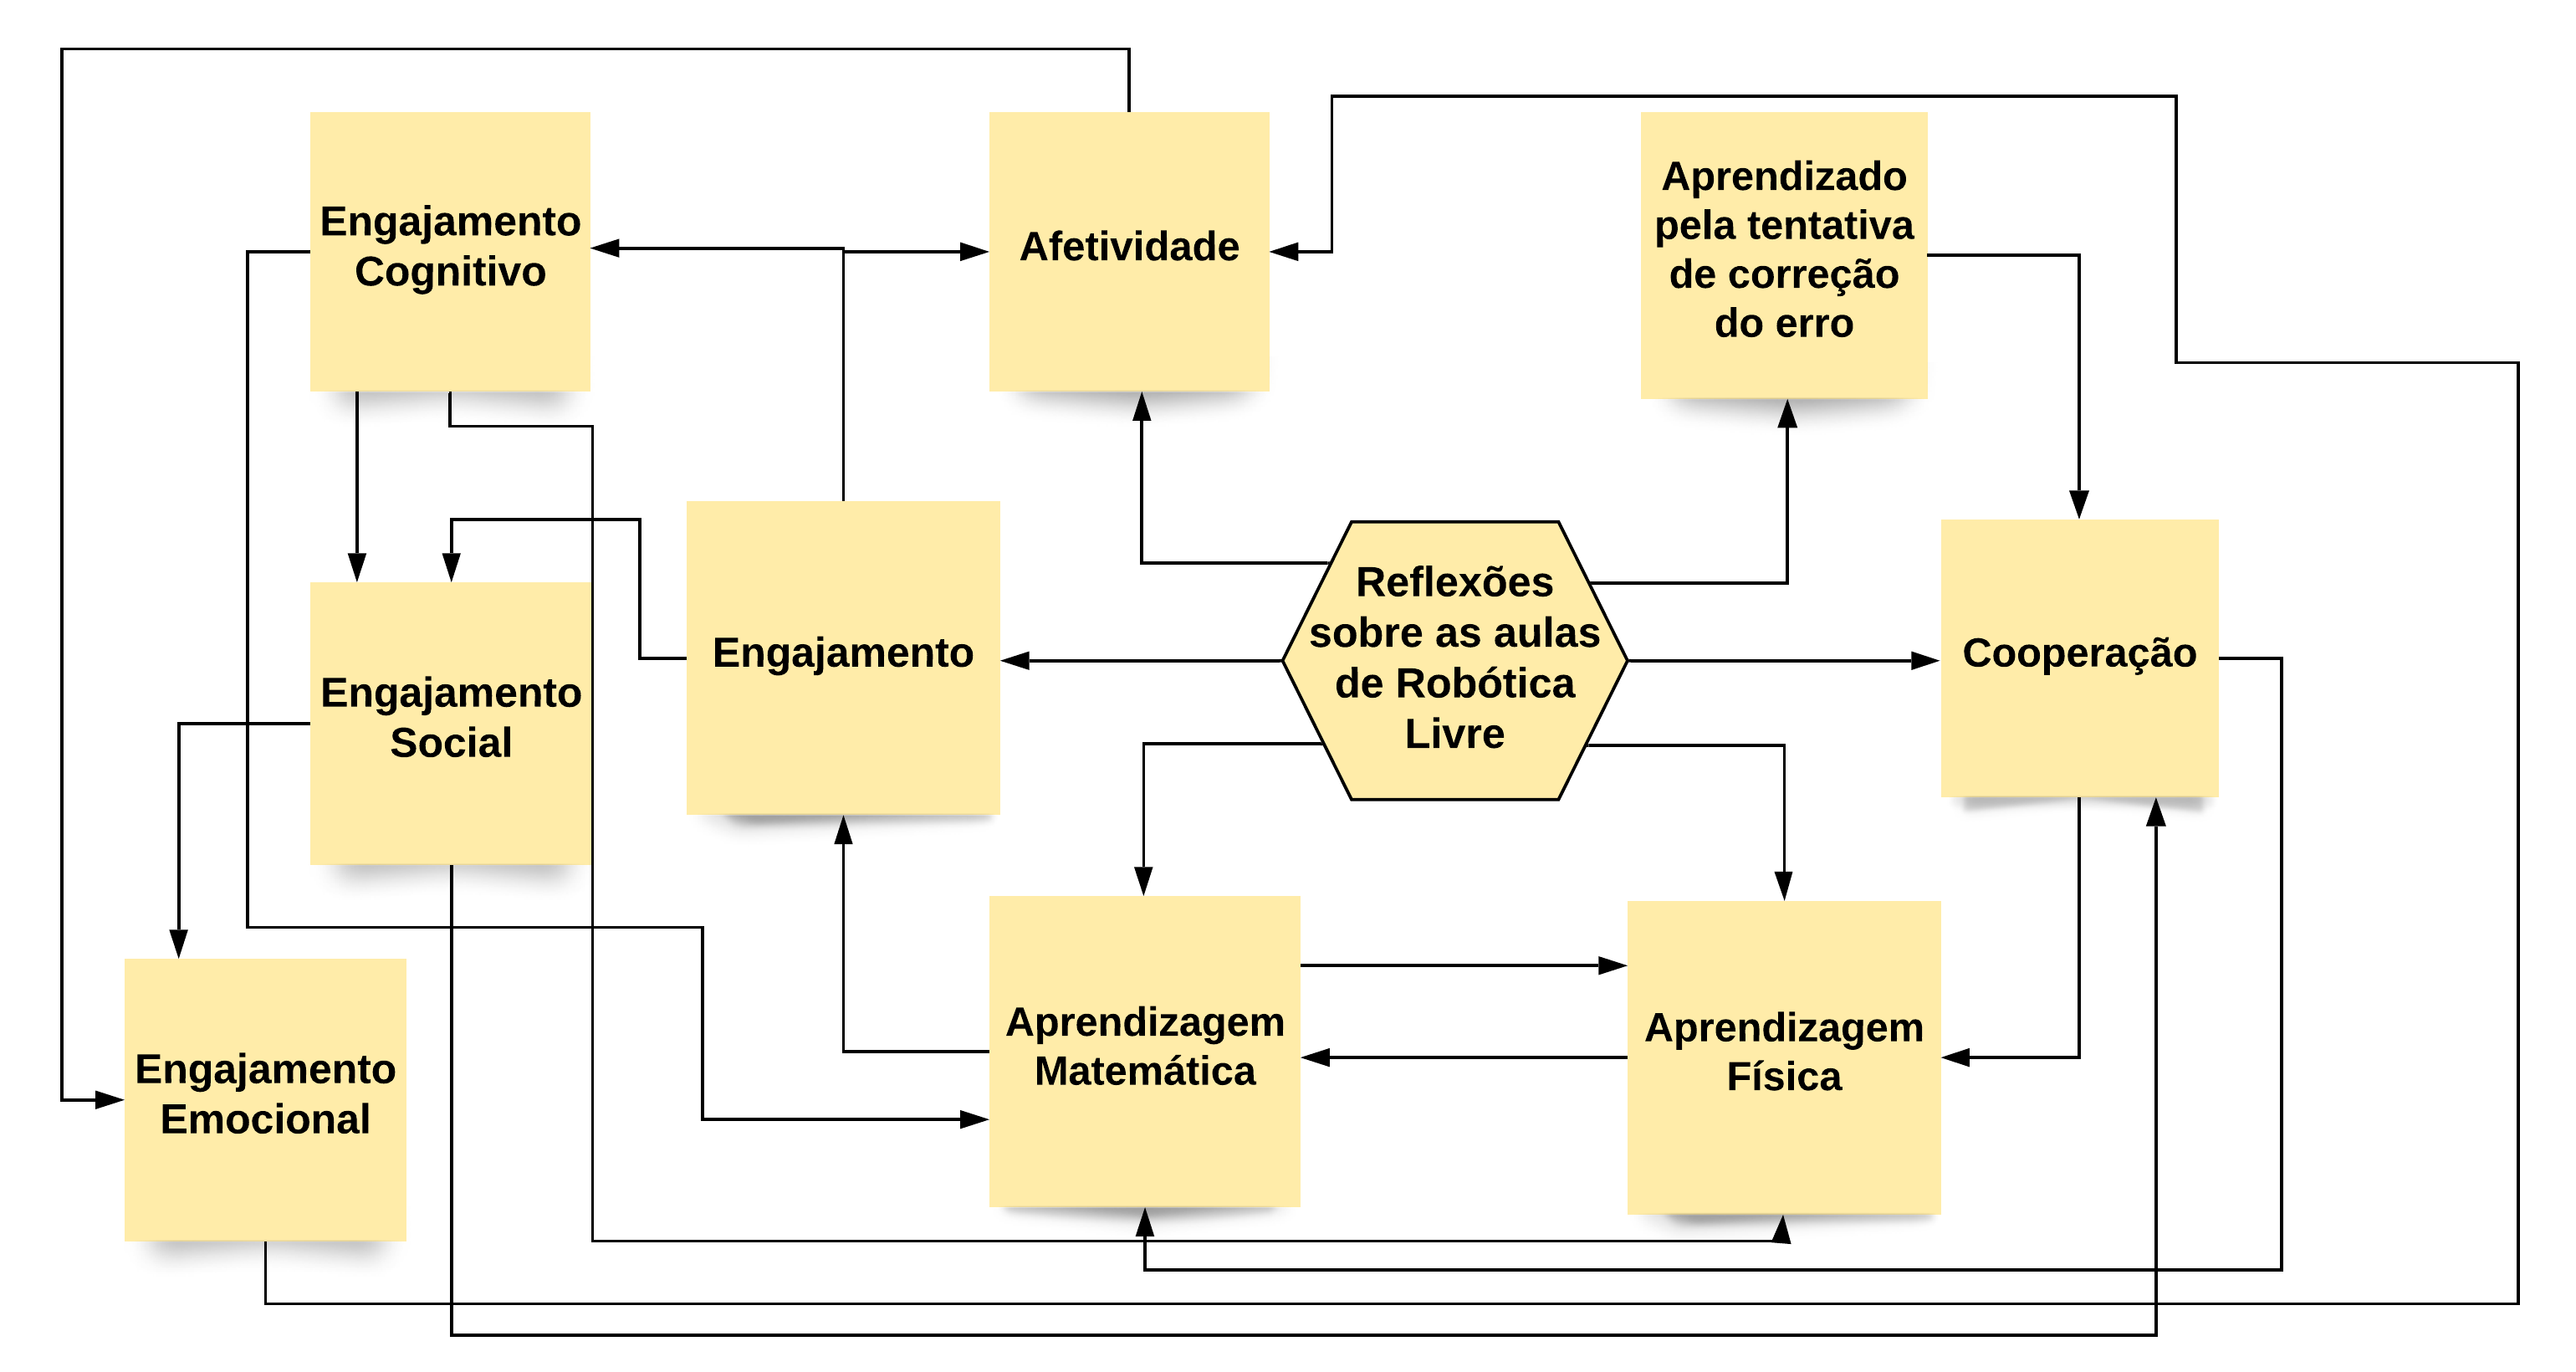
\includegraphics[width=0.9\textwidth]{fig-017.png}
 \caption{Correlações entre o desenvolver da atividade de Robótica Educacional Livre, sentimentos e aprendizagem.}
 \label{fig17}
 \source{Arquivo pessoal.}
\end{figure}

Os participantes, ao realizarem a montagem do robô, mobilizavam várias habilidades, dentre elas a atenção. A atenção é uma habilidade importante para desenvolvimento cognitivo e pessoal humano, bem como para o desenvolvimento da robótica. Quando não realizamos algo com atenção, estamos suscetíveis ao erro. Mas, dentro da presente proposta objeto de investigação da pesquisa, observamos que o erro também é importante e faz parte do desenvolvimento de outras habilidades. Com o erro, os participantes procuraram corrigi-lo, aprofundado o seu conhecimento em detalhes pertinentes ao robô. 

O aparecimento do erro promove o engajamento social entre os participantes que, por consequência, leva ao engajamento emocional e a algo marcante (experiência), como nos diria o autor \textcite[p. 21]{larrosa2002}: “a experiência é o que nos passa, o que nos acontece, o que nos toca”.

Observamos que o aprendizado acontece nessa perspectiva, por meio da montagem do robô, com ou sem erro. Este último promove o engajamento social entre os participantes, que leva ao engajamento emocional, promovendo o aprendizado Matemático e Físico nas entrelinhas do desenvolvimento dos robôs. 

Quando os participantes não conseguem desenvolver a montagem dos robôs, o professor pode ou não interferir no processo. Se o professor optar por não interferir diretamente no processo, ele pode orientar ou dar uma direção, de como o participante pode obter a resposta, ou dar dicas de como conseguir realizar a montagem. Por outro lado, caso o professor interfira diretamente, ele pode fazer questionamentos sobre a montagem aos participantes. O ato de realizar esses questionamentos, em nossa visão, promove o engajamento cognitivo, reforçando as ideias e os aprendizados internalizados pelos participantes, ressaltando a atenção. Quando esses questionamentos resultam em alguma ideia de ação, os participantes tendem a cooperar e compartilhar seus resultados, entrando novamente no ciclo da espiral de aprendizagem criativa, proposta por \textcite{resnick2020}.

\section{Considerações finais}\label{sec-5}
Considerando a utilização da Robótica Educacional Livre, aliada ao construcionismo de \textcite{papert1980, papert2008}, por meio de sequências de montagens de robô, observamos os conhecimentos desenvolvidos e criados, que permeiam seu desenvolvimento por meio da espiral de aprendizagem criativa  apresentada por \textcite{resnick2020}. Acreditamos que a Robótica Educacional Livre tem um grande potencial para ser uma aliada ao processo de aprendizagem  das disciplinas de Matemática, Física, Computação, Engenharias e Arte, observando a adequação do conhecimento que se deseje construir, ao desenvolver das sequências didáticas dos robôs.

Para trabalhos futuros, podemos buscar quais seriam os resultados para um grupo de participantes maior, bem como o que poderíamos obter de resultados em outras turmas, como, por exemplo, um grupo de participantes de Ensino Médio. Para projetos futuros, por meio da utilização do Arduino e sensor ultrassônicos, vislumbramos a possibilidade da criação de um robô para o cálculo de área e o volume de um espaço, que pode ser no formato de paralelepípedo, como uma sala de aula, ou o volume de um cone, pirâmide, permitindo o trabalho com a Geometria Espacial.

No presente contexto, essa proposta de projetos futuros pode ser talvez um resultado de uma construção de conhecimento, que perpassa a espiral de aprendizagem criativa, pois,  após a criação de robôs que realizavam cálculo de distância e velocidade do som em determinado ambiente,  surgiu a ideia de aplicabilidade em cálculo de área e volume.

Outros projetos desenvolvidos na pesquisa permitiram a criação de algumas ideias e aplicações com os componentes presentes nos \textit{kits} adquiridos. Com o sensor de temperatura com NTC, por meio do modelo de equação Steinhart–Hart, poderá ser criado um termômetro digital para diversos fins, seja apenas para quantificar a temperatura ambiente, seja para um estudo mais aprofundado de temperatura de determinada localidade. Como o modelo de Steinhart-Hart envolve funções logarítmicas neperianas, talvez seu estudo se dê melhor no Ensino Médio. Outra possibilidade de trabalho com temperatura e umidade dá-se através do sensor DHT-11,  que pode medir tanto a temperatura quanto a umidade relativa do ar. Em projetos anteriores, criamos um robô de controle de umidade e temperatura de ambiente, com um umidificador de ar e um ventilador, quando pudemos estudar vários modelos, como, exemplo, maximizar o uso de energia no resfriamento e umidificação de ambientes. 

Com o sensor de umidade de solo, podemos criar um robô para o controle de umidade para plantas e desenvolver, a partir disso, modelos de utilização de água para sua economia e maximização pela(s) planta(s) para determinada cultura/lavoura irrigada.

Com o sensor infravermelho, podemos utilizar  um controle remoto para o controle de determinado projeto, para que ocorra seu controle presencial sem fio. Outra possibilidade refere-se à criação de um sistema hidropônico utilizando Arduino, fazendo uso do controle de temperatura e acionamento de bomba d’água, com possibilidade de medição de condutividade elétrica e PH, da solução hidropônica, tornando o processo mais tecnológico e automatizado, e fazendo com que diminuam os prejuízos de manejo.
 
Essas ideias podem ser compartilhadas com professores e adeptos, uma vez que idealizamos a proposta de desenvolvimento de novas sequências de montagem com a visão de adaptar o currículo comum, utilizando-se da ciência do aprendizado, a matética.

Por meio dos relatos dos participantes e pelas tecnologias utilizadas na pesquisa, concluímos que os participantes criaram ideias do que gostariam de construir. Embora não tenhamos aprofundado nas ideias por falta de tempo, observamos que os participantes chegaram à Espiral de Aprendizagem Criativa, defendida por \textcite{resnick2020},  desenvolvendo conhecimentos através de um ciclo, que leva a imaginar, criar, brincar, compartilhar, refletir, imaginar, mas não necessariamente nessa ordem, pois os estudantes podem criar algo, por exemplo, a partir de uma sequência de montagem, e, por meio dela, começar a imaginar novas possibilidades e invenções.

Através dessas experiências, podemos fazer emergir conceitos de Matemática e Física, com a construção de robôs, proporcionando a constituição de um ambiente de ensino e aprendizagem diferente de um modelo tradicional, em que podemos trabalhar o conhecimento curricular tradicional, criando situações motivadoras e contextualizadas.

\printbibliography\label{sec-bib}
% if the text is not in Portuguese, it might be necessary to use the code below instead to print the correct ABNT abbreviations [s.n.], [s.l.] 
%\begin{portuguese}
%\printbibliography[title={Bibliography}]
%\end{portuguese}


%full list: conceptualization,datacuration,formalanalysis,funding,investigation,methodology,projadm,resources,software,supervision,validation,visualization,writing,review
\begin{contributors}[sec-contributors]
\authorcontribution{Marcelo Pires da Silva}[datacuration,writing,funding,conceptualization,formalanalysis]
\authorcontribution{Fernando da Costa Barbosa}[supervision,writing,methodology,datacuration,conceptualization]
\end{contributors}

\end{document}
